\textbf{Dreamfusion}~--~This method initiates the modeling process with a random scene initialization, which it then incrementally refines throughout the training period. A unique aspect of this method is that each prompt triggers the formation of a new scene, ensuring that even when the same textual input is used repeatedly, it results in the creation of distinct objects. This feature of Dreamfusion is showcased through the results visible in Figure~\ref{fig:generationDreamFusion} and Figure~\ref{fig:secondRobotDreamfusion}, both of which are included in the Appendix.
For the purposes of this research, the stable-DreamFusion variant \citep{stable-dreamfusion}, as available in Threestudio, was utilized. This version is distinct from the original Dreamfusion implementation, primarily due to the unavailability of Imagen to the public. Details regarding any other modifications made in this version, compared to the original, are outlined in the Appendix. 

\begin{figure}[H]
    \centering
    % Subfigure for textual description
    \begin{subfigure}[b]{0.20\textwidth}
        \centering
        \fontsize{9pt}{7pt}\selectfont\text{Iteration = 100}\vspace{3cm}
        \fontsize{9pt}{7pt}\selectfont\text{Iteration = 5000}\vspace{2.85cm}
        \fontsize{9pt}{7pt}\selectfont\text{Iteration = 10000}\vspace{1.95cm}
    \end{subfigure}
    \begin{subfigure}[b]{0.20\textwidth}
        \centering
        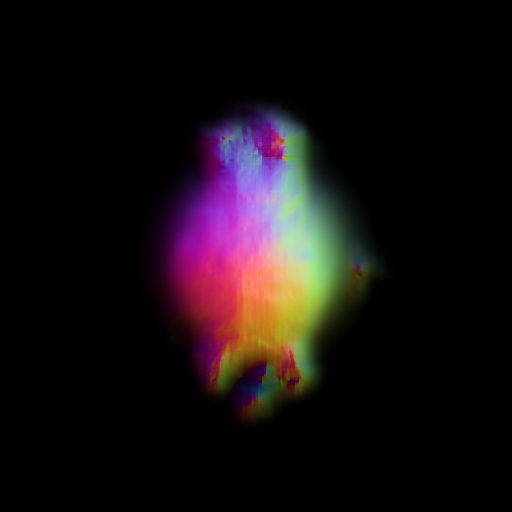
\includegraphics[width=\textwidth]{etc/a robot made out of plants/dreamfusion/dreamfusion_plantrobot_1_part2.png}
        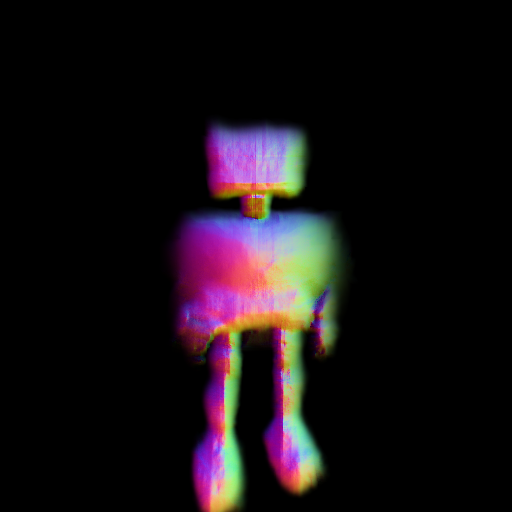
\includegraphics[width=\textwidth]{etc/a robot made out of plants/dreamfusion/dreamfusion_plantrobot_5000_part2.png}
        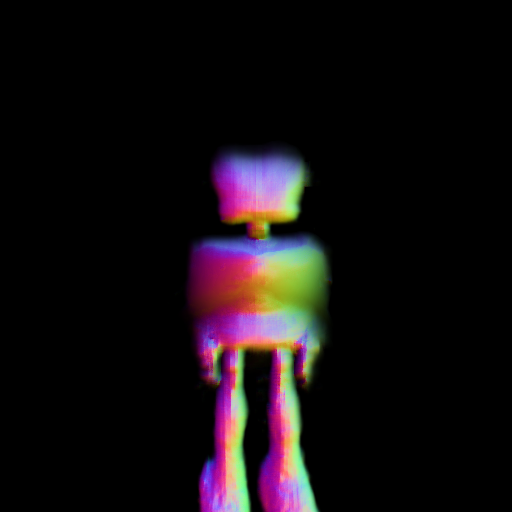
\includegraphics[width=\textwidth]{etc/a robot made out of plants/dreamfusion/dreamfusion_plantrobot_10000_part2.png}
        \caption{}
    \end{subfigure}
    \begin{subfigure}[b]{0.20\textwidth}
        \centering
        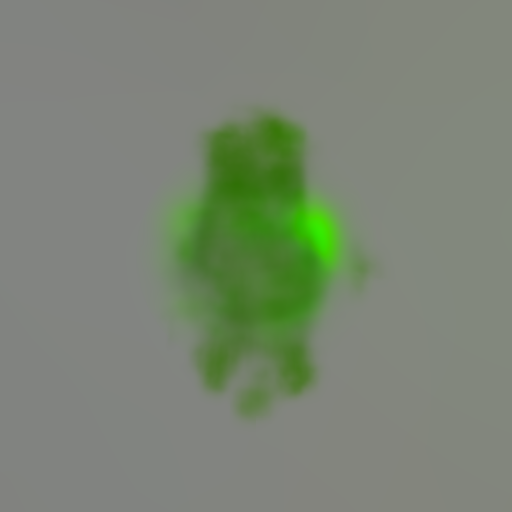
\includegraphics[width=\textwidth]{etc/a robot made out of plants/dreamfusion/dreamfusion_plantrobot_1_part1.png}
        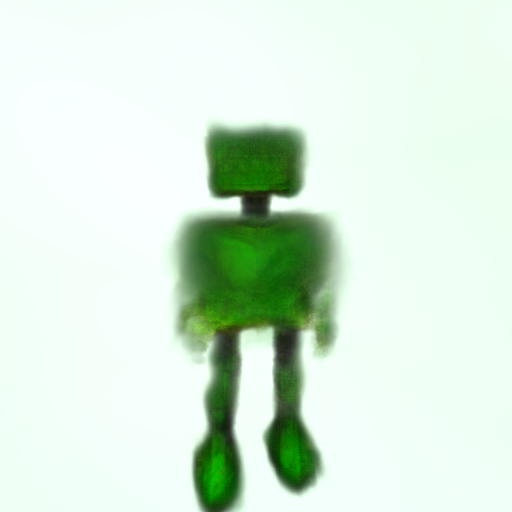
\includegraphics[width=\textwidth]{etc/a robot made out of plants/dreamfusion/dreamfusion_plantrobot_5000_part1.png}
        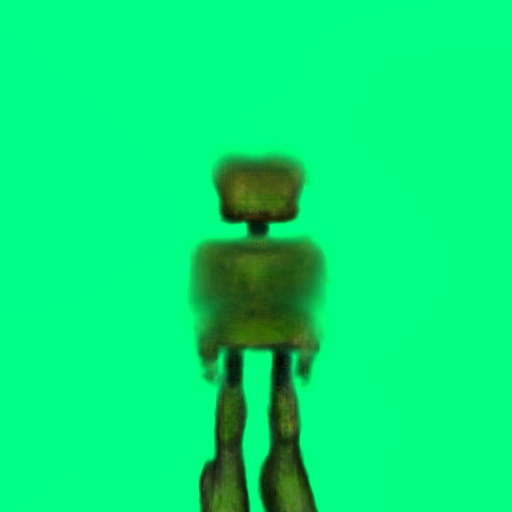
\includegraphics[width=\textwidth]{etc/a robot made out of plants/dreamfusion/dreamfusion_plantrobot_10000_part1.png}
        \caption{}
    \end{subfigure}
    % Subfigure 3
    \hspace{.5cm}
    \begin{subfigure}[b]{0.252\textwidth}
        \centering
        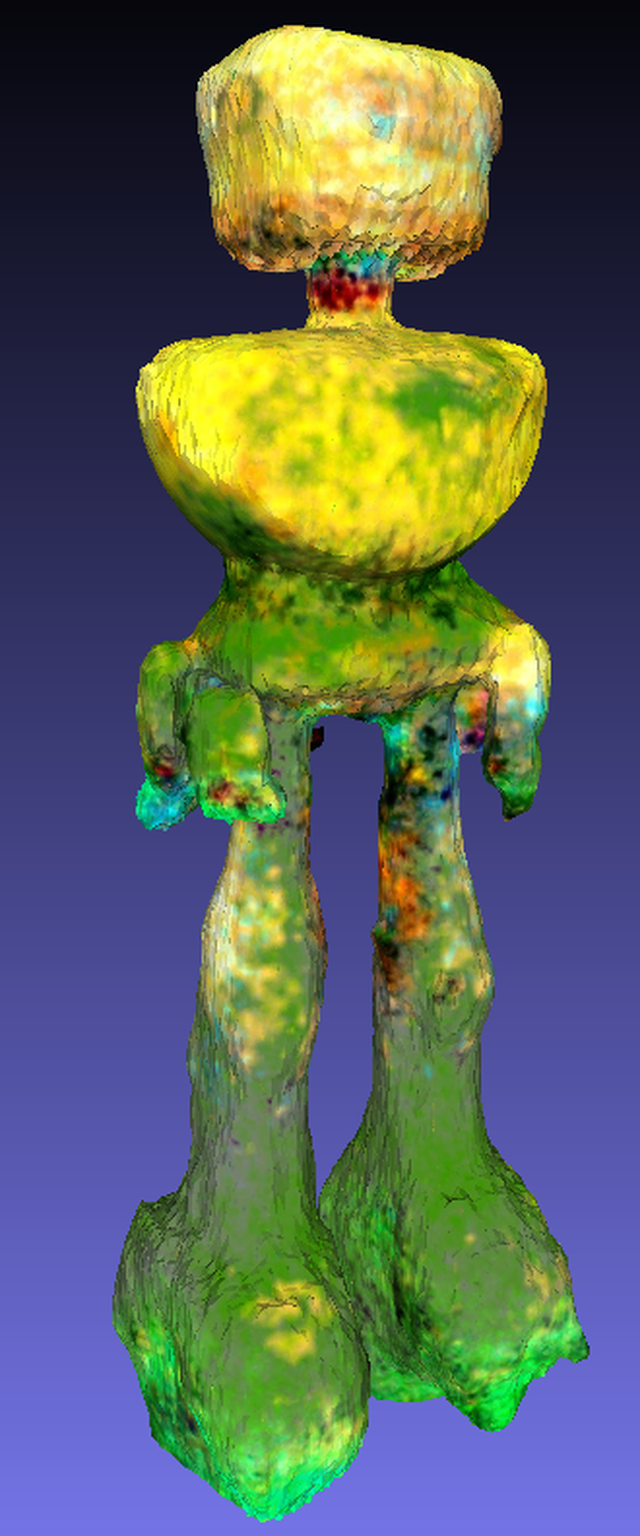
\includegraphics[width=\textwidth]{etc/a robot made out of plants/dreamfusion/dreamfusion_plantrobot_model_resized.png}
        \caption{}
    \end{subfigure}
    \caption{The generation process of Dreamfusion using the prompt ``a robot made out of plants''. Section (c) shows a snapshot of the final mesh generated.}~\label{fig:generationDreamFusion}
\end{figure}

As seen in Figure~\ref{fig:generationDreamFusion} parts (a) and (b), the object and its texture are generated simultaneously. The process starts with a small dot that gradually transforms into a more complex shape. At the 100th iteration, the original dot begins to transform into a recognizable shape, and a green hue resembling plant coloration is created. At the 5000th iteration, distinct features such as two legs, a square body and a square head become visible, all retaining the same shade of green. At the last, 10,000th iteration, the model shows a background and small arms sticking out of the robot's body.
Part c of the figure showcases the rendered mesh opened in Meshlab \citep{meshLab}, highlighting alterations made by Threestudio, such as duplicate removal and hole filling. These modifications account for the slight differences between the final mesh and the validation images produced during training. Interestingly, the final mesh lacks detailed plant-like features, one could only assume that the legs kind of resemble moss, but this remains speculation. The mesh primarily shows basic shapes, including a square head, a torso with small protruding rods that could be arms, and large legs. Remarkably, the upper half of the body in the final mesh takes on a yellowish color that differs from the green of the earlier validation images. The reason for this color change remains unclear.\newline